\subsection{Boltzmann machine learning}
\begin{itemize}
	\item Unsupervised learning problem
	\item We want the maximize the product of the probabilities that the Boltzmann machine assigns to the binary vectors in the training set
	\item Equivalent to maximizing the sum of the log probabilities that the Boltzmann machine assigns to the training vectors
	\item It is also equivalent to maximizing hte probability that we would obtain exactly the N training cases if we did the following:
	\begin{itemize}
		\item Let the network settle to its stationary distribution N different times with no external input
		\item Sample the visible vector once each time
	\end{itemize}

	\subsubsection{Why the learning could be difficult}
	\item Consider the chain of units:
	\begin{center}
		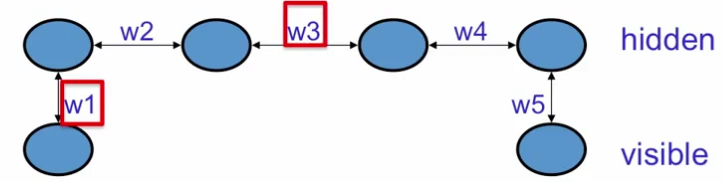
\includegraphics[scale=0.6]{sections/12/chain.png}
	\end{center}
	\item If the raining set consists of (1,0) and (0,1) we want the product of all the weights to be negative (So to know how to change w1 or w5 we must know w3)

	\item Everything that one weight needs to know about the other weights and the data is contained in the difference of two correlations:
	\begin{center}
		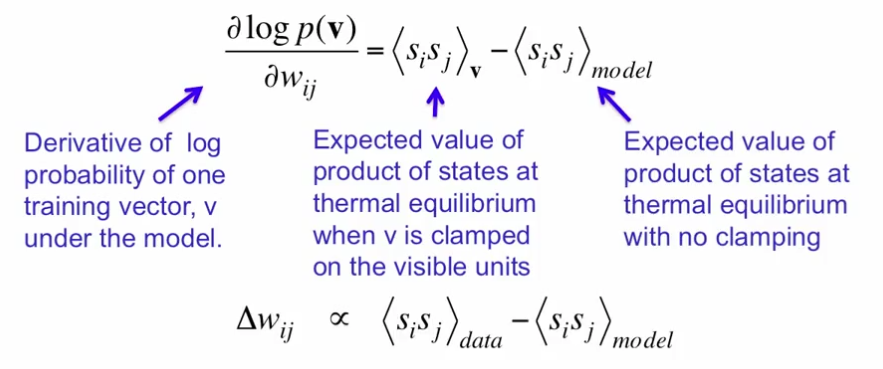
\includegraphics[scale=0.6]{sections/12/corr.png}
	\end{center}
		$$\delta w_{ij} \propto \langle s_i s_j \rangle_{data} - \langle s_i s_j \rangle_{model}$$

	\subsubsection{Why is the derivative so simple?}
	\item THe probability of a global configuration at thermal equilibrium is an exponential function of its energy
	\item So setting to equilibrium makes the log probability a linear function of the energy
	\item The energy is a linear fnuction of the weights and states, so:
		$$-\frac{\partial E}{\partial w_{ij}}=s_i s_j$$

	\item The process of settling to thermal equilibrium propagates information about the weights (We dontt need backprop)

	\subsubsection{Why do we need the negative phase?}
	\item Probability of a visible vector:
	\begin{center}
		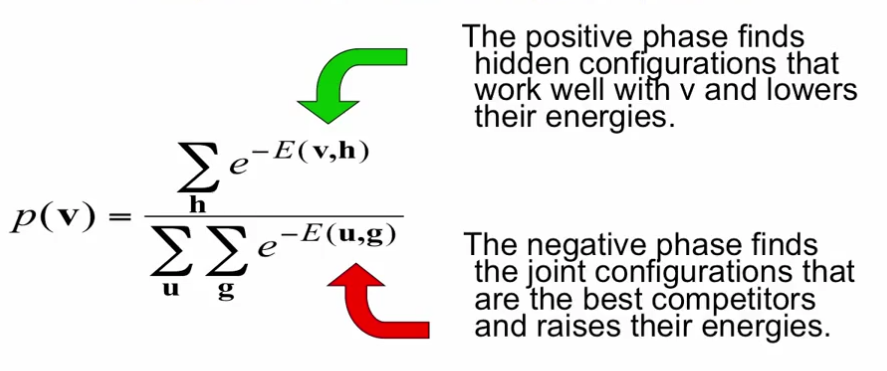
\includegraphics[scale=0.6]{sections/12/neg.png}
	\end{center}

	\subsubsection{An inefficient way to collect the statistics required for learning}
	\item \textbf{Positive phase}: clamp a data vector on the visible units and set the hidden units to random binary states
	\item Update the hidden units one at a time until the network reaches thermal equilibrium at a temperature of 1
	\item Once equilibrium, Sample $s_i s_j$ for every connected pair of units
	\item Repeat for al ldata vectors in the training set and average
	\item \textbf{Negative phase}: Set all the units to random states
	\item Update until equilibrium at temperature of 1
	\item Sample $s_i s_j$ for every connected pair of units
	\item Repeat many times and average to get good estimates
\end{itemize}